\chapter{Git}\label{git-explanation}
In this chapter the \ac{vcs} \emph{Git} will be introduced.
As Git is the foundation of this thesis, I will explain user roles, technologies, internal data representations and other relevant parts of Git.


\section{Introduction to Git}\label{git-introduction}
Git is a tool, which is used to manage different versions of files in a specific directory.
Each version of the project is saved as a so called \emph{commit}.
Users are able to meticulously specify the files or changes in files that should be added to a commit.
It is also capable of showing the exact changes between different commits, which is called a \emph{diff}.

Git is the currently most popular tool to control a project's code with an still trending tendency~\footnote{Version Control Systems Popularity in 2016~\url{https://rhodecode.com/insights/version-control-systems-2016} Retrieved Jan. 22, 2018}.
It enables to work with multiple developers on a single code base, as it provides several different techniques, the \emph{history tree}, the \emph{branch} and the \emph{merge}.
The versioning history of Git is internally represented as an directed, non-cyclic, connected graph of commits or a \emph{tree}.
The commits act as \emph{nodes} and the connection to their parent commits as \emph{edges}.
Every time two edges leave a single node, a new \emph{branch} is created.
In Git, every branch has its own name, whereby the main branch is usually named \emph{master}.

\begin{figure}[h]
    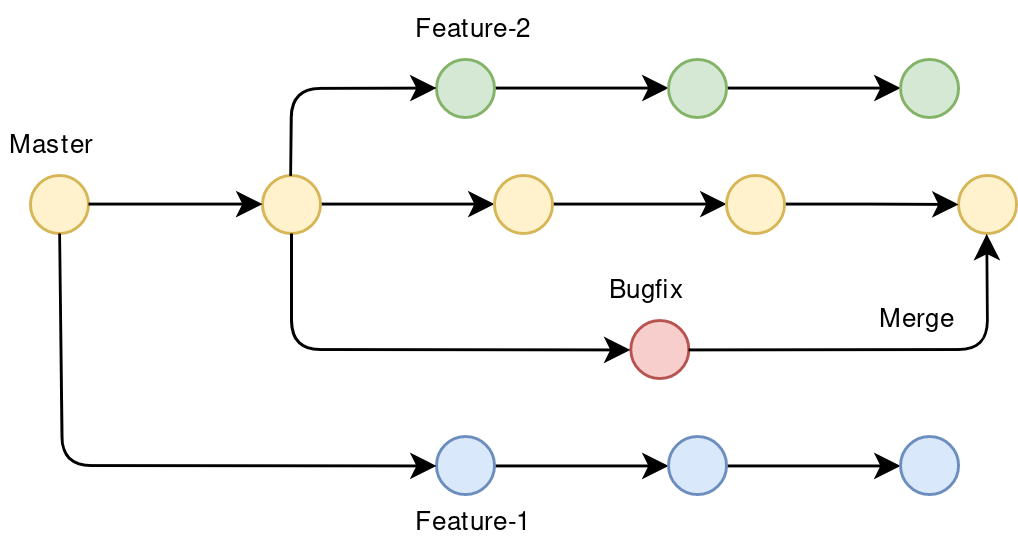
\includegraphics[scale=0.4]{./graphs/git-history-branch}
    \centering
    \caption{A Git commit history tree.}\label{fig:git-commit-tree}
\end{figure}

In case two different people want to work on the same files, they can each create their own branch on which they can work unimpeded.
After they finished and want to add their work to the master branch, they can now \emph{merge} their changes.
Git then tries to automatically resolve any conflicts which might have emerged from editing the same lines in a file.
If that is not possible, it marks the conflicts and allows the user to manually correct them.


With this methodology it is possible to work with many people or teams on the same project without accidentally overwriting changes of another developer whilst maintaining a clear history of all changes of the project.

Another important feature of Git is the \emph{remote}.
A remote is usually located on a distinct server, which is attached to some kind of network, which is accessible by developers.
A remote acts as a single source of truth a developer can \emph{push} their changes to or \emph{pull} changes from other developers.
Git supports several protocols such as \ac{http} or \ac{ssh} to connect to the remote and to provide a simple user management layer.


\section{Git User Roles}
There exist two roles in Git, namely the \emph{committer} and the \emph{author}.
Every commit in Git contains the email addresses and the names of these two people.
The \emph{author} of a commit is the person which actually contributed the changes in the files.
The \emph{committer} is the person, which created the git commit.
This is important to keep track of the original author of the changes.

Lets look at the case of an author contributing code to a project in an email with an attached patch file.
If a maintainer of the project now applies the patch file and commits without setting the \emph{author}, the information about the original author would be lost.
Although in most cases the \emph{author} and the \emph{committer} are the same person. \todo{Prozentzahl auf Basis der gesammelten Daten.}


\section{Internal Representation}
Git provides a collection of high level abstraction tools to work with it's underlying \ac{fs}.
In the following I'll explain the structure and management of Git's \ac{fs}.

The most basic structure in Git is a \emph{blob} object.
A \emph{blob} object is any file, which has been added to a Git \ac{fs}.
It is compressed and saved in the \inlinecode{.git/objects} directory under the respective \ac{sha1} hash of the uncompressed file.
As follows there exists a blob object for every version of every file of the project.

The \ac{sha1} hashing for unique file identifier might seem unsafe, but the probability of a \ac{sha1} collision is really low, roughly $10^{-45}$.
Lately Google managed to force a collision in an controlled environment in 2017, but it is really unlikely to encounter a collision under normal circumstances.~\footnote{Announcing the first SHA1 collision:~\url{https://security.googleblog.com/2017/02/announcing-first-sha1-collision.html} Retrieved Dec. 16, 2017}.
This feature of \ac{sha1} hashing become quite important in the design of the database later on.

As mentioned in the introduction\ref{git-introduction} Git is used to store the state of a specific directory on any underlying \ac{fs}.
To represent a \ac{fs} or to simply bundle multiple Git \emph{blob} objects together, Git uses the \emph{tree} object.

A \emph{tree} object is a file, which has a \ac{sha1} hash reference to all underlying \emph{blob} and \emph{tree} objects as well as their names and file permissions.
To represent a subdirectory a \emph{tree} simply holds a reference to another \emph{tree} object.

\begin{minted}[linenos]{text}
    100644 blob 11d1ee77f9a23ffcb4afa860dd4b59187a9104e9  .gitignore
    040000 tree ac0f5960d9c5f662f18697029eca67fcea09a58c  expose
    100644 blob 61b5b2808cc2c8ab21bb9caa7d469e08f875277a  install.sh
    040000 tree 8aaf336db307bdcab2f082bd710b31ddb5f9ebd4  thesis
\end{minted}
\begingroup
\captionof{listing}{\emph{tree} file example\label{lst:raw-commit}.}
\endgroup

As stated before the \emph{commit} is utilized to provide an exact representation of a state of the repository's files and directories.

\begin{minted}[linenos]{text}
    tree      cd7d001b696db430b898b75c633686067e6f0b76
    parent    c19b969705e5eae0ccca2cde1d8a98be1a1eab4d
    author    Arne Beer <arne@twobeer.de> 1513434723 +0100
    committer Arne Beer <arne@twobeer.de> 1513434723 +0100

    Chapter 2, acronyms
\end{minted}
\begingroup
\captionof{listing}{\emph{commit} file example\label{lst:raw-commit}.}
\endgroup

As you can see in listing~\ref{lst:raw-commit}, the \emph{commit} is just another kind of file utilized by Git, which contains some meta data about a repository version:

\begin{itemize}
    \item The reference to a \emph{tree} object, which represents the root directory of the project.
    \item A reference to one or multiple parent commits, to maintain a version history.
    \item The name and email address of the author.
    \item The name and email address of the committer.
    \item The \ac{utc} timestamps with \ac{utc} offset for the commit and author date.
    \item The commit message. A message with arbitrary text from the committer.
\end{itemize}

Just as the \emph{blob} object the \emph{tree} and \emph{commit} files are also stored in the \inlinecode{.git/objects} directory under their respective hash.
With these methods it is now possible to jump between different versions by calling \inlinecode{git checkout \$hash} with the version commit hash or to create a \emph{diff} between two commits with \inlinecode{git diff \$hash1 \$hash2}.
